\begin{exercise}
      {ID-2f20460e1c1d42ddf8ddbe4e06d9a23c1485cefe}
      {Mittelwerte}
  \ifproblem\problem\par
    Untersuche, ob eine der folgenden Aussagen für alle positiven Zahlen $a,b$ gilt:\par
    \begin{minipage}{0.44\textwidth}
      \centering
      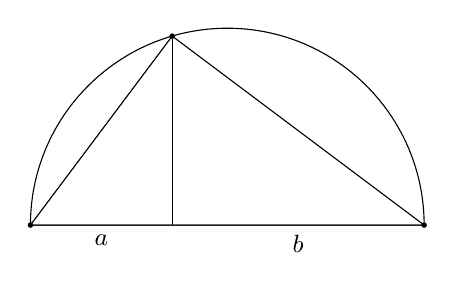
\begin{tikzpicture}
        \coordinate (A)  at ( 0mm,  0mm);
        \coordinate (B)  at (50mm,  0mm);
        \coordinate (C)  at (18mm, 24mm);
        \coordinate (F)  at (18mm,  0mm);
        % Eckpunkte
        \fill (A) circle (1pt);
        \fill (B) circle (1pt);
        \fill (C) circle (1pt);
        % Dreieck
        \draw (A) -- (B) -- (C) -- cycle;
        % Hoehe
        \draw (C) -- (F);
        % Halbkreis
        \draw (A) -- (B) arc (0:180:25mm);
        % Beschriftung
        \path (A) -- node[below] {{\small$a$}} (F);
        \path (F) -- node[below] {{\small$b$}} (B);
      \end{tikzpicture}
    \end{minipage}%
    \hfill
    \begin{minipage}{0.55\textwidth}
      \begin{enumerate}[a)]
        \item $\displaystyle\frac{a+b}{2}\leq\sqrt{ab}$
        \item $\displaystyle\frac{a+b}{2}\geq\sqrt{ab}$
        \item $\displaystyle\frac{a+b}{2}\neq\sqrt{ab}$
      \end{enumerate}
    \end{minipage}
  \fi
  %\ifoutline\outline\par
  %\fi
  %\ifoutcome\outcome\par
  %\fi
\end{exercise}
